% $Id: chapter1.tex 1790 2010-09-28 16:46:40Z jabriffa $

\chapter{Introduction}

\section{Dissertation Format}
This template is provided to facilitate the process of writing up your
dissertation while ensuring its format is consistent with requirements.
In using this template, \emph{do not}, under any circumstances, make any
changes to the class file provided.
In particular, do not attempt to make any changes to the title page, the
statement of originality, or the copyright page.

Use of this template is not mandatory; if you choose not to use it, then you
must make your final layout resemble this output as closely as possible.
In particular, the textual content and layout of the title page, statement of
originality, and copyright page must not be changed.

\section{Using \LaTeX{}}

\subsection{Supported platform}
The supported platform for this template is a system with:
\begin{itemize}
\item An Ubuntu 10.04 operating system
\item The \verb|texlive-full| package installed
\end{itemize}
This setup is available at least in the Duck/Swan labs, and is supported by
FEPS IT.
The template itself is kept as simple as possible, to facilitate its use on
other systems.

The template also assumes the installation of the GNU make system.
To compile the template into a PDF, simply issue the \verb|make| command
in the template folder, from a terminal.

\subsection{Adding figures}
The simplest way to add figures is to use the \verb|graphicx| package, as shown
in the example that produces Figure~\ref{fig:sample}.
\LaTeX{} automatically finds a suitable place to lay out the figure.
A number of graphic formats are supported -- please refer to the package
documentation for further details.

\begin{figure}[tp]
   \begin{center}
      \subfigure[Diagrammatic representation]{
         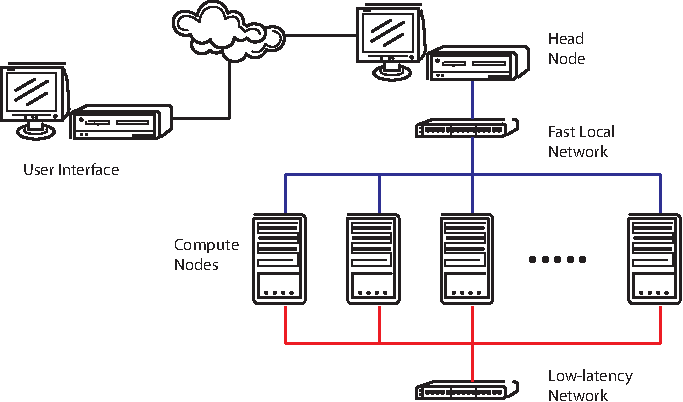
\includegraphics{Figures/cluster}
         }
      \subfigure[Photo of the Tempest cluster]{
         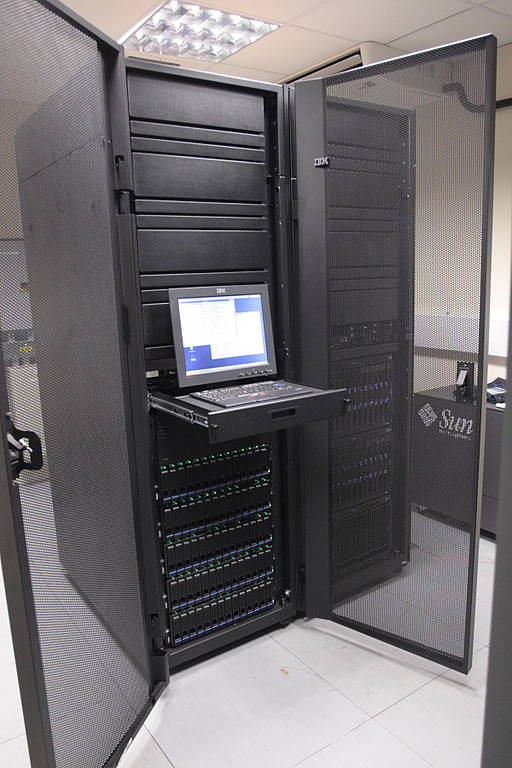
\includegraphics{Figures/tempest}
         }
   \end{center}
   \caption{An example figure, with two parts}
   \label{fig:sample}
\end{figure}

\subsection{Adding tables}
Tables are handled in a similar way to figures, although in this case the text
is entered directly in the source file.
An example is given in Table~\ref{tab:sample}.

\begin{table}[tp]
   \begin{minipage}{\textwidth}
      \begin{center}
         \begin{tabular}{l|c}
            Operation            & Speed \\
            \hline
            Add, Mul, Mul-Add    & 8 \\
            Reciprocal           & 2 \\
            Divide               & 0.88 \\
            Divide Intrinsic     & 1.6 \\
            \hline
            Recip.\ Square Root  & 2 \\
            Square Root          & 1 \\
            \hline
            Logarithm            & 2 \\
            Exponent             & 1 \\
            \hline
            Sin, Cos Intrinsics  & 2 \\
            Sin, Cos, Tan        & Slow \\
         \end{tabular}
      \end{center}
   \end{minipage}
   \caption{An example table, showing speed in operations per cycle per
   multiprocessor}
   \label{tab:sample}
\end{table}
  
\subsection{Adding equations}
One of the strong points of \LaTeX{} is its formatting of mathematical notation.
It can easily handle numbered equations, as in the recursive formula:
\begin{equation}
\alpha(\iota,x_2) = \sum_{x_1,d_{\iota-1}} \alpha(\iota-1,x_1)
   \prob{ \vec{r}_{n(\iota-1)+x_1,n\iota+x_2}, \vec{t}_{\iota-1} }
\end{equation}
or math within the main body of text, for example to specify $1 \leq \iota
< N$.
More complex equations are also handled with ease, as in the following case,
where the equation is too long to fit in a single line:
\begin{equation}
\prob{\vec{r}_{0,n\iota+x_2}, \varsigma_{n\iota}=x_2}
= \sum_{x_1,d_{\iota-1}} \left[
\begin{split}
   & \prob{\vec{r}_{0,n(\iota-1)+x_1}, \varsigma_{n(\iota-1)}=x_1} \\
   & \times \prob{ \vec{r}_{n(\iota-1)+x_1,n\iota+x_2}, \vec{t}_{\iota-1} }
\end{split} \right]
\end{equation}

\subsection{Adding code fragments}
Code fragments in \LaTeX{} can be added using the \verb|verbatim| environment,
as shown in the example below.
Remember to set the line spacing as shown, or you'll end up with double-spaced
code listings.

\singlespaced
\begin{verbatim}
typedef int v4si __attribute__ ((vector_size (16)));

void ArrayAdd(int *c, const int *a, const int *b, int n)
   {
   const v4si *va = (const v4si *)a;
   const v4si *vb = (const v4si *)b;
   v4si *vc = (v4si *)c;
   int i = 0;
   if(n > 4)
      for(; i < n / 4; i++)
         vc[i] = va[i] + vb[i];
   for(i *= 4; i < n; i++)
      c[i] = a[i] + b[i];
   }
\end{verbatim}
\doublespaced

\subsection{Adding references}
One of the more convenient facilities provided by \LaTeX{} is the handling of
references using \BibTeX.
This allows you to completely separate the bibliography database from the
citations within the text, and more importantly from the way these are
formatted.
\BibTeX support a number of reference types; examples are given in this
template for:
\begin{itemize}
\item Conference papers \cite{bsw10icc}
\item Journal articles \cite{gamal}
\item Dissertations \cite{tunstall}
\item Books \cite{press}
\item User or technical manuals \cite{cuda-pg,netpbm}
\item Technical Reports \cite{bw1994}
\item Other material that cannot be easily classified \cite{farrell}
\end{itemize}
\subsection{Rough Structure}
Abstract - Explain brief overview of what the aim is. Automatically generate API clients for microservices to use to communicate with one another whilst ensuring that contractually all information is sent/received as expected (additional benefit of 
allowing languages like typescript to pull out the API resposne type etc)

Introduction - motivation for it at hindsight. Talk about microservice stack, whilst utilising typescript its a pain to have to manually create a service local client for calling the other service endpoints - follow on to how its time consuming to manually create
the response types within the consumer service (so the logic knows the contents of the JSON response etc). Potentially talk about using OpenAPI spec (Swagger) over last couple years (might be better in lit review though)

Objectives - see email

Structure/outline of the report - needs clarification

Lit review
	- Further in depth analysis of problem. More technical and broader - not necessarily MY experience in this one
	- Use my case study of why it would be helpful, saves time on actual code writing, but also essentially acts as small unit tests on the code as long as the language is strongly typed etc.
	/// NOT SURE ON ORDER HERE -> FOLLOWING IS WHAT I FEEL IS LOGICAL - worth a discussion though I guess, if order actually matters?
	- Brief introduction to microservices - why what how. How does typical client/server model fit into the relationships between multiple microservices. Client service requests an endpoint from the server service etc
	- Talk about what modern clients need to handle (maybe talk about serverside too, but two sides of the same coin essentially). Rate limiting, error handling, pagination etc, why is this sort of scalabilty
	important etc. What are general best practises
	- Talk about API specifications in general -> float into OpenAPI/Swagger - what other options are there (vague research for filler). Benefits of using it etc. =
	- Talk about general code generation. Move onto the specific OpenAPI/Swagger CodeGen tooling - maybe a bit of background on the tech they use in it - out of scope though or extra flavour?

Requirements and Specifications
	- Pull out actual tangible goals from Objectives? User stories - see BDD and Gherkin spec language - can also pull into why its used - shill for Hindsight etc
	- Explain each of the following end products
		- Example microservice with the TSOA library - uses decorator patterns to create the Open API spec directly from the Controller layers. Additonal libraries for getting a functional service 
		up and running but essentially they have little bearing on the actual project itself. Unit test libraries etc but again this is just flavour. End result is a microservice that can generate
		its API spec on command
		- Once the service is built, create a generic client for consuming its endpoints. Just a blank template - utilise best practises from the lit review. Unit tested, use of aditional libraries
		for handling some of the heavier options. Want lightweight code for later on in the code gen.
		- When the client meets its reqs use it as a template for the swagger codegen. All this entail is modifiying the files within the codegen library and expanding their logic with all of the
		additional functionality from our client. Essentially pulling out the code and writing it in the Mustache templating language so that the different vars can be filled out when the microservice spec
		is applied to it.
	- Not entirely sure what it wants for the SDLC Methodologies - this seems like a typical buzzword net. I guess I just say im doing agile cus everything else sucks? Despise this sorta documentation so needs clarification

System Design
	- How am I using Agile etc. Could look at setting up a Jira project etc, but all of this seems like a bit of a waste of time as I'll essentially ignore it and do it after the software is finished. Might be worth it 
	for the marks though. Thoughts?
	- Design experiments - could talk about anaylsis of different libraries - this will be more like a thought experiment/analysis though - unclear if this covers what it wants?
	- Everything else like details of design decisions - will comprehensive Git history with proper messages cover this? I can also talk about code structure and general design I've picked up as I've tweaked the Hindsight services 
	etc. Seems to also feed in from library decisions etc as well as why I'm using the CodeGen solution etc. Real want to avoid doing UML etc, makes me wanna cry.

Testing/Validation
	- Unit Tests and pull back into User Stories from Reqs. Could go full TDD and write Integration/Acceptance tests but that's a lot of effort and I don't think it's worth it really - maybe at end if time?
	- Evaluate each of the stages - is microservice stable, do tests pass etc? If I write in a basic database system can have it fetching queries etc and talk about that here. Is the Spec file it generates correct.
	Is it easy to use. Same sort of thing for the client, does it fulfil the best practises from the lit review - see unit tests too. Does the code generated from my templates work as expected, could look at testing the unit tests
	from the original template against it - sort of acts as an end to end test - worth looking into. 
	- Generic evaluation on end results vs objectives themselves

Conclusions
	- Was it a success - talk about test results etc?
	- What was actually achieved. Tie back into why I wanted it, how will it be integrated into Hindsight if it's successful enough etc.
	- Future work - I'll look for inspiration when I get to this.
